\chapter{Modelos de Redes Neurais}
\label{ch:03}


% \epigraph{\itshape Those who cannot remember the past are condemned to compute it.''}{---Steven Pinker, \textit{Words and Rules}}

Este capítulo serve como uma introdução à teoria das Redes Neurais. Os conceitos aqui introduzidos servirão como embasamento teórico imprescindível para a apresentação do modelo final utilizado nesta pesquisa, o \textit{Encoder-Decoder}. 

\section{Aprendizado de Máquina}
\label{sec:ml}

Um modelo de rede neural é, essencialmente, um modelo de aprendizado de máquina supervisionado (\cite{Goodfellow-et-al-2016})
que está a procura de identificar padrões. Um modelo de aprendizado de máquina é uma tarefa computacional que explora algoritmos que podem aprender a partir de seus erros e fazer previsões sobre dados. Os possíveis tipos de aprendizado de máquina são divididos entre: \textit{supervisionados}, \textit{não-supervisionados}
e por \textit{reforço} (\cite{Gron:2017}). 

Os aprendizados não-supervisionados podem ser caracterizados pela não utilização dos \textit{alvos} durante o treinamento. Eles são tipicamente utilizados para tarefas de classificação. A Figura \ref{fig:iris} mostra um exemplo de classificação não-supervisionada realizada com a utilização do \textit{dataset “Iris”} (\cite{Dua:2019}). O \textit{dataset} é composto por colunas de diferentes características analisadas em três espécies diferentes de plantas. O algoritmo de aprendizado não-supervisionado utilizado foi o \textit{K-means} (\cite{Shalev-Shwartz:2014:UML:2621980}). A proposta do aprendizado não-supervisionado é deduzir predições possíveis a partir da identificação de grupos (\textit{clusters}) que compartilham de características similares. Na figura, é possível observar que há um grupo de observações cujo o tamanho das pétalas e das sépalas é em geral menor que os demais (grupo \textit{amarelo}), isto pode indicar que estas observações sejam de uma mesma espécie. Os grupos \textit{azul} e \textit{marrom} não apresentam uma separação clara entre si, isto pode tornar a tarefa de classificação mais complicada. Chamam a atenção três pontos dispersos à direita. Estas observações não parecem pertencer a nenhum dos grupos formados. Elas podem ser observações ditas \textit{outliers}, observações muito discrepantes que podem ser um indício de erro durante a coleta dos dados ou apenas indivíduos que escapam a uma distribuição típica (\cite{2004:bussab}). 

\begin{figure}[!htb]
    \center{\includegraphics[width=0.7\textwidth]
    {img/iris.png}}
    \caption{\label{fig:iris} Algoritmo não-supervisionado (K-means) realizado no \textit{dataset Iris} }
  \end{figure}

Os aprendizados por reforço consistem em algoritmos que recebem sinais de recompensa/punição quando acertam/erram uma tarefa de interesse. Recomenda-se a leitura de \cite{KLMSurvey:1996} para maiores detalhes.

um paragrafo maior sobre aprendizado supervisionado, tarefas de regressao etc
No caso das redes neurais, o aprendizado diz-se supervisionado, pois informa-se ao modelo o \textit{alvo} esperado  pelo treinamento para cada informação de entrada (Fig. \ref{fig:gabarito}). 

\section{Introdução Teórica a Redes Neurais}
\label{sec:intro-rn}
A inspiração para o desenvolvimento da modelagem em Redes Neurais Artificiais surgiu a partir de estudos em neurosciência que concluíram que, diante de múltiplas apresentações de um mesmo estímulo, um mesmo conjunto de neurônios sofre incitação e dispara. Um estímulo diferente resulta no disparo de um conjunto de neurônios diferente (\cite{hubel:1962}).  Analogamente, o modelo artificial é composto por uma camada denominada de \textit{input} responsável por receber diferentes estímulos (matematicamente retratados por vetores numéricos que representam o objeto do aprendizado). A informação recebida é distribuída ao longo de múltiplas conexões com a próxima camada através de uma multiplicação com uma matriz de pesos $\vect{W}$ (Fig. \ref{fig:diagram}). A matriz de pesos funciona como uma analogia às conexões existentes entre neurônios de modo que um peso maior (mais próximo de 1) representa uma conexão reforçada e um peso menor (mais próximo de 0) representa uma conexão reprimida. Na figura estão representados três pesos como exemplos, porém na prática, todas as conexões tem pesos associados.

% Suponha uma arquitetura simples com um \textit{input} de dimensão 3. Dada essa suposição, o número de linhas da matriz $W$ fica condicionado a 3 para que a multiplicação seja possível. O número de colunas da matriz depende da dimensão da próxima camada. Para ilustrar, suponha novamente que a dimensão da próxima camada também tem dimensão 3. Algebricamente, o processo descrito é representado pela multiplicação apresentada em \ref{eq:mult}.

% \begin{equation}
% \label{eq:mult}
%   \begin{bmatrix}
%     x_1\\
%     x_2\\
%     x_3\\
%   \end{bmatrix}
%   \cdot
%   \begin{bmatrix}
%     w_{(1,1)} & w_{(1,2)} & w_{(1,3)} \\
%     w_{(2,1)} & w_{(2,2)} & w_{(2,3)} \\
%     w_{(3,1)} & w_{(3,2)} & w_{(3,3)} \\
%   \end{bmatrix} 
% \end{equation}

\input{definitions/colors}
\input{definitions/styles}
\begin{figure}[H]
\centering

\scalebox{1.0}{
\begin{tikzpicture}[auto]

\node[textonly] (1pho1) {1};
\node[textonly, below=45pt of 1pho1] (1pho2) {0};
\node[textonly, below=45pt of 1pho2] (1pho3) {0};

% Legenda
\node[textonly, above=20pt of 1pho1] (leg1) {Inputs};
\node[textonly, right=55pt of leg1] (legw) {Matriz de Pesos \textbf{W}};



% FNN input
\node[normal, right=25pt of 1pho1] (x1) {};
\node[normal, below=45pt of x1] (x2) {};
\node[normal, below=45pt of x2] (x3) {};

\node[text, below=5pt of x1] (nada) {};
\node[textonly, right=13pt of nada] (w12) {0.4 };
\node[textonly, below=36pt of w12] (w11) {0.8};

\node[textonly, below=70pt of w12] (w32) {0.2};
%\node[textonly, left=1pt of nada] (w31) {0.2 $w_{(3,1)}$};

\node[text, below=10pt of x3] (nada) {};

% FNN output
\node[box2, right=95pt of x2] (y2) {$\displaystyle\Sigma$};

% edges FNN
\path[tedge] (x1) -- (y2);

\path[tedge] (x2) -- (y2);

\path[tedge] (x3) -- (y2);

\node[box2, right=30pt of y2] (activation) {$f$};

\node[text, right=40pt of activation] (output) {$\hat{y}$};

\node[text, right = 40pt of legw] (lego) {\textbf{Output}};



\path[tedge] (y2) -> (activation);

\path[tedge] (activation) -> (output);

\end{tikzpicture}
}\caption{Digrama de uma Rede Neural do Tipo Perceptron} 
\label{fig:diagram}
\end{figure}  

O resultado dessa multiplicação gera um vetor, cujos valores são em seguida somados ($\displaystyle\Sigma$). O valor resultante entra como argumento em uma função (que nesse contexto é chamada de \textit{função de ativação} ($f$)). As funções de ativação são parte fundamental do funcionamento da rede, são elas que permitem o aprendizado de relações complexas (não lineares) entre os \textit{inputs} e os \textit{alvos}. 

Uma das funções de ativação mais utilizadas na literatura (e inclusive utilizada pelos pesquisadores Rumelhart e McClelland) é a função \textit{Sigmoid}, uma função com propriedades matemáticas desejáveis e que comprime os resultados obtidos em um intervalo de [0, 1]. Tal compressão possibilita a associação dos \textit{outputs} do modelo a probabilidades. A Fig. \ref{fig:sigmoidplot} mostra o gráfico da função \textit{Sigmoid}. Na literatura existem ainda outras funções comumente utilizadas, como a \textit{ReLu}, a \textit{Tanh} e a \textit{Softmax}
(\cite{Goodfellow-et-al-2016}). A escolha dessas funções depende da tarefa em que estão sendo aplicadas. Entretanto, o ajuste dos modelos de Redes Neurais é bastante experimental. Na prática, recomenda-se consultar a literatura por tarefas similares para realizar tal escolha. Na ausência de tarefa similar, as funções tem seus desempenhos comparados para que se decida por uma delas. 

\begin{figure}[H]
\centering
\scalebox{0.9}{
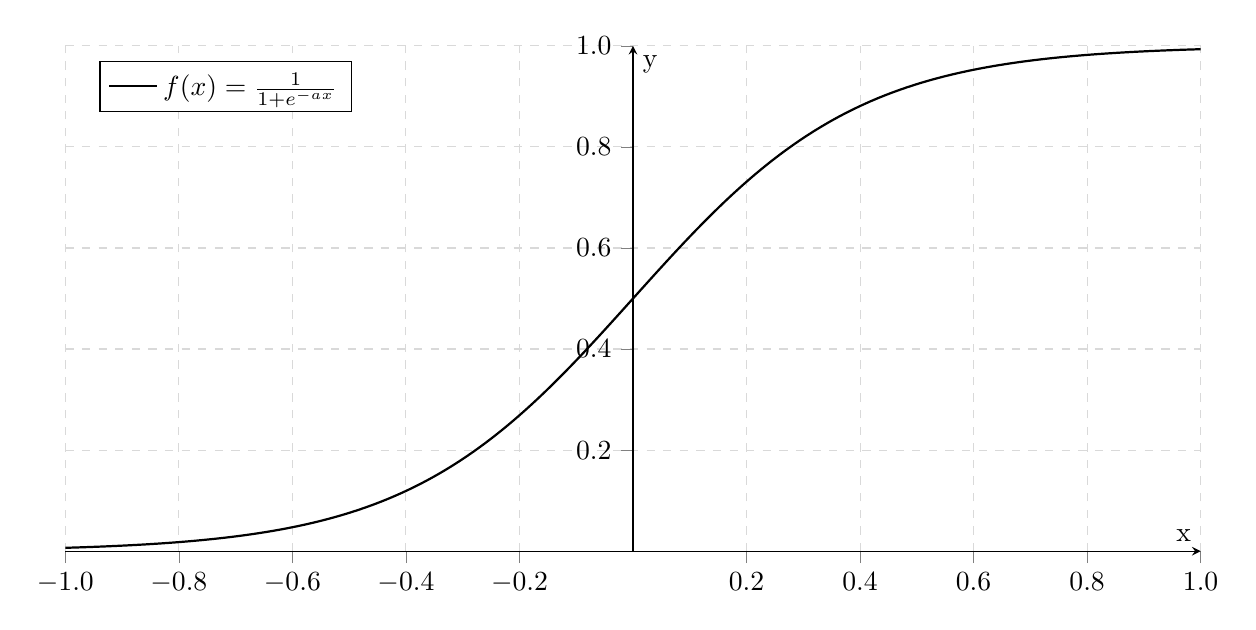
\begin{tikzpicture}
    \begin{axis}[
    	legend pos=north west,
        axis x line=middle,
        axis y line=middle,
        x tick label style={/pgf/number format/fixed,
                            /pgf/number format/fixed zerofill,
                            /pgf/number format/precision=1},
        y tick label style={/pgf/number format/fixed,
                            /pgf/number format/fixed zerofill,
                            /pgf/number format/precision=1},
        grid = major,
        width=16cm,
        height=8cm,
        grid style={dashed, gray!30},
        xmin=-1,     % start the diagram at this x-coordinate
        xmax= 1,    % end   the diagram at this x-coordinate
        ymin= 0,     % start the diagram at this y-coordinate
        ymax= 1,   % end   the diagram at this y-coordinate
        %axis background/.style={fill=white},
        xlabel=x,
        ylabel=y,
        tick align=outside,
        enlargelimits=false]
      % plot the stirling-formulae
      \addplot[domain=-1:1, black, thick,samples=500] {1/(1+exp(-5*x))};
      %\addplot[domain=-1:1, blue, ultra thick,samples=500] {1/(1+exp(-10*x))};
      \addlegendentry{$f(x)=\frac{1}{1+e^{-ax}}$}
      %\addlegendentry{$g(x)=\frac{1}{1+e^{-10x}}$}
    \end{axis} 
\end{tikzpicture}
}
\caption{A função \textit{Sigmoid}.}
\label{fig:sigmoidplot}
\end{figure} %diminuir esse desenho

 O diagrama apresentado na Fig. \ref{fig:diagram} representa uma arquitetura conhecida como \textit{Perceptron}. Essa arquitetura, uma das primeiras construídas, é bastante simples. O \textit{Perceptron} consiste de um vetor de \textit{inputs}, uma matriz de pesos, uma função de ativação e um \textit{output} (\cite{Rosenblatt:1957}). 
 
 A partir dessa estrutura, as arquiteturas das Redes Neurais foram se tornando mais complexas, com por exemplo a adição de uma ou mais camadas intermediárias, antes da camada de \textit{output}. Tais camadas intermediárias são chamadas de \textit{camadas escondidas} (Ver Fig. \ref{fig:ffd}.).

% \begin{align}\label{eq:sigmoid}
% p(w_{i} = 1) = \frac{1}{1+e^{\sum_{i} w_{i}x_{i}}}
% \end{align}

% Algebricamente, pode-se representar o processo descrito através da composição de múltiplas funções, uma vez que o resultado das operações precedentes servirão como entrada para as próximas camadas.

% \begin{align}
% % f(\vect{x}) &= f^{(2)}(f^{(1)}(\vect{x}; \vect{W}_1); \vect{W}_2)\\
% % &= 
% \sigma(\vect{W}_2 (\sigma(\vect{W}_1\vect{x})))
% \end{align}

\input{definitions/colors}
\input{definitions/styles}
\begin{figure}[ht!]
\centering

\scalebox{1.0}{
\begin{tikzpicture}[auto]

% operations =========

% FNN input
\node[normal] (x1) {};
\node[textonly, above=10pt of x1] (input) {Camada de \textit{inputs}};
\node[normal, below=10pt of x1] (x2) {};
\node[normal, below=10pt of x2] (x3) {};
\node[normal, below=10pt of x3] (x4) {};
\node[normal, below=10pt of x4] (x5) {};
\node[normal, below=10pt of x5] (x6) {};

% FNN output
\node[textonly, right=50pt of x1] (center) {Camada Escondida};
\node[normal, below=25pt of center] (y1) {};
\node[normal, below=10pt of y1] (y2) {};
\node[normal, below=10pt of y2] (y3) {};

% FNN output
\node[textonly, right=110pt of input] (output) {Camada de \textit{outputs}};
\node[normal, below=15pt of output] (z1) {};

\node[normal, below=10pt of z1] (z2) {};
\node[normal, below=10pt of z2] (z3) {};
\node[normal, below=10pt of z3] (z4) {};
\node[normal, below=10pt of z4] (z5) {};
\node[normal, below=10pt of z5] (z6) {};

% phon features 2

% edges FNN
\path[nedge] (x1) -- (y1);
\path[nedge] (x1) -- (y2);
\path[nedge] (x1) -- (y3);

\path[nedge] (x2) -- (y1);
\path[nedge] (x2) -- (y2);
\path[nedge] (x2) -- (y3);

\path[nedge] (x3) -- (y1);
\path[nedge] (x3) -- (y2);
\path[nedge] (x3) -- (y3);

\path[nedge] (x4) -- (y1);
\path[nedge] (x4) -- (y2);
\path[nedge] (x4) -- (y3);

\path[nedge] (x5) -- (y1);
\path[nedge] (x5) -- (y2);
\path[nedge] (x5) -- (y3);

\path[nedge] (x6) -- (y1);
\path[nedge] (x6) -- (y2);
\path[nedge] (x6) -- (y3);

% edges FNN
\path[nedge] (y1) -- (z1);
\path[nedge] (y1) -- (z2);
\path[nedge] (y1) -- (z3);
\path[nedge] (y1) -- (z4);
\path[nedge] (y1) -- (z5);
\path[nedge] (y1) -- (z6);
\path[nedge] (y2) -- (z1);
\path[nedge] (y2) -- (z2);
\path[nedge] (y2) -- (z3);
\path[nedge] (y2) -- (z4);
\path[nedge] (y2) -- (z5);
\path[nedge] (y2) -- (z6);
\path[nedge] (y3) -- (z1);
\path[nedge] (y3) -- (z2);
\path[nedge] (y3) -- (z3);
\path[nedge] (y3) -- (z4);
\path[nedge] (y3) -- (z5);
\path[nedge] (y3) -- (z6);

\end{tikzpicture}
}\caption{Esquema de uma Rede Neural com Camada Escondida} 
\label{fig:ffd}
\end{figure}

Como comentado na Seção \ref{sec:compmot}, o acréscimo das camadas escondidas aumenta a capacidade de aprendizado dos modelos. Isso acontece porque a cada camada intermediária, o modelo aprende a identificar características relevantes para a produção de uma resposta final (o \textit{output}). É como se cada uma delas fosse responsável pela identificação de traços importantes diferentes. Como exemplo, considere as características relevantes para a identificação de uma espécie de animal: Para identificá-lo, é relevante saber o tamanho do animal, se ele tem penas, pelos ou cartilagem; se tem quatro patas, etc.  
Entretanto, no modelo de Redes Neurais, é difícil determinar quais informações estão sendo mais relevantes para a aprendizagem. Deve-se lembrar que o modelo funciona através de vetores numéricos, representações que se tornam cada vez mais abstratas conforme a profundidade (número de camadas) aumenta.

\section{Treinamento}

Na Seç. \ref{sec:ml} falamos sobre o fato de uma Rede Neural ser um aprendizado de máquina supervisionado. Para que a rede seja capaz de identificar os padrões desejados, é necessário provê-la com os \textit{alvos}), pois o treinamento da mesma consiste, essencialmente, na atualização das matrizes de pesos que deve ocorrer a partir da comparação entre os valores previstos pela rede (os \textit{outputs}) e os \textit{alvos}. A comparação entre esses valores se dá por meio de uma função de custo (\textit{Loss Function}), que representa uma forma de se quantificar o quão perto se está de uma rede ideal em que os resultados previstos correspondam exatamente aos \textit{alvos}. O objetivo do aprendizado da rede é minimizar essa diferença, ou seja, encontrar os valores dos pesos na matriz $\vect{W}$ que minimizam a função de custo (\cite{josh:2017}). Para isso, faz-se uso de um algoritmo chamado de \textit{backpropagation} (\cite{Goodfellow-et-al-2016}). Após a inserção de cada input e a aplicação do algoritmo de backpropagation, todos os pesos são atualizados simultaneamente com os valores que em conjunto minimizam a função de custo, e portanto, aproximam as previsões da rede aos alvos. Entretanto, o ajuste de um modelo de redes neurais é bastante delicado e experimental. Ele depende não somente da busca pelos melhores valores para os pesos da matriz $W$ como também de uma busca pelos chamados \textit{hiperparâmetros}. 

Os hiperparâmetros são parâmetros do modelo que são escolhidos a priori para sua configuração. Um deles refere-se ao número de vezes em que um mesmo \textit{input} é inserido, conhecido como o número de \textit{épocas}. O treinamento de uma Rede Neural, se dá por meio de \textit{ciclos}. Cada vez que um mesmo \textit{input} é apresentado a rede, ocorre uma nova predição, e consequentemente, uma nova comparação com o \textit{alvo}. Desse modo, a rede tem a oportunidade de ir refinando e ajustando os pesos para que os \textit{outputs} se aproximem dos \textit{alvos}.

Já foi falado um pouco sobre a quantidade de camadas intermediárias. Como essa questão determina a arquitetura da rede, também deve ser definida a priori, sendo considerada também um hiperparâmetro. Ademais, a dimensionalidade (número de nódulos) de tais camadas também deve ser pré-determinada. 

Existem também outros hiperparâmetros importantes como a taxa de aprendizado $\eta$, o parâmetro de regularização $\lambda$, taxa de \textit{Dropout}, entre outros (\cite{josh:2017}). Todos esses hiperparâmetros definem as configurações do modelo.

Sobre a determinação dos hiperparâmetros, esta não é uma tarefa trivial, visto que há uma variedade de hiperparâmetros que podem ser combinados de várias maneiras. Múltiplos treinamentos com diferentes configurações de hiperparâmetros são realizados para que se possa fazer essa escolha. Na prática, porém, é mais comum que esses hiperparâmetros sejam configurados a partir de resultados de experimentos semelhantes publicados na literatura. Existem também algoritmos de exploração de hiperparâmetros, como por exemplo o \textit{Grid Search}. Dado um conjunto de hiperparâmetros para teste, este algoritmo testa todas as combinações possíveis e devolve como solução a combinação que gerou o melhor resultado (\cite{Goodfellow-et-al-2016}).

Mesmo com uma extensa busca pelos hiperparâmetros do modelo, nem sempre é possível encontrar valores em $\vect{W}$ que possibilitem o aprendizado de forma satisfatória. Na prática, é bastante comum a ocorrência de problemas conhecidos como \textit{overfit} (quando o modelo se torna especialista nos dados de treino mas tem dificuldade de generalizar para dados nunca vistos antes) e \textit{underfit} (quando o modelo falha em capturar o padrão subjacente dos dados) (\cite{josh:2017}). Na literatura existem algumas técnicas disponíveis para tratar dessas questões, como \textit{Dropout}, \textit{Data Augmentation} e \textit{Resampling} (\cite{Goodfellow-et-al-2016}, \cite{josh:2017}).  %ref 

\section{Uma Outra Arquitetura}
\label{sec:arqFDD}

No Capítulo \ref{ch:02} exploramos dois tipos de pré-processamentos de verbos: (i) O processo de codificação de \cite{rumelhart:1986}, que fazia uso de tríades de traços fonéticos para manter um registro de ordem sequencial dos \textit{inputs}, e (ii) o pré-processamento escolhido para alimentação do modelo \textit{Encoder-Decoder} desta pesquisa.

Como comentado, a arquitetura do \textit{Encoder-Decoder} é mais adequada do que a \textit{Feedforward} para a inserção de dados de comprimentos variáveis. Isso é possível graças a uma arquitetura composta por \textit{Redes Neurais Recorrentes}.

Antes, porém, da apresentação desta arquitetura, faz-se necessária uma introdução ao conceito de \textit{Modelo de Linguagem}.

\subsection{Modelo de Linguagem}

Um modelo de linguagem é um modelo que propõe uma distribuição probabilística para uma sequência de termos em uma linguagem natural (\cite{Manning:1999}).
Dessa forma, é possível estipular um termo mais provável dada uma sequência de termos anteriores (um histórico). Como exemplo, suponha um dado histórico, como: “\textit{Pedro vai à \_\_\_}”. Com um modelo de linguagem, poderemos completar a frase com novos termos, como: “\textit{missa}”, “\textit{praia}”, “\textit{festa}”, etc. A resposta para tal questão dependerá basicamente do modelo de linguagem proposto e principalmente do corpus no qual o modelo foi treinado. 

Modelos de linguagem são fundamentais para inúmeras aplicações computacionais rotineiras. Os casos de uso mais intuitivos são os serviços de auto-preenchimento, bastante utilizados em aplicativos de celulares para trocas de mensagens de texto. Entretanto, também são utilizados para correção automática, transcrição de áudio para texto,  tradução automática, entres outros.  

Para entender como os modelos de linguagem são obtidos, começaremos formalizando a questão que tentam responder, ou seja, atribuir uma probabilidade a um termo \textbf{t} dado um histórico \textbf{h}, isto é, propor uma $P(t \mid h)$. Pode-se representar uma sequência de $N$ termos como $t_1, t_2, t_3, ..., t_n$. Assim, a probabilidade que queremos computar agora pode ser escrita como a probabilidade conjunta $P(t_1, t_2, ..., t_n)$. Considera-se também o \textbf{histórico} como sendo a sequência $t_1, t_2, ..., t_{n-1}$ ou também, de forma simplificada, $t_{1}^{k-1}$. 

Seguindo a regra da cadeia para probabilidades (\cite{Jurafsky:2009:SLP:1214993}), podemos decompor a probabilidade conjunta que queremos utilizando a seguinte fórmula:

\begin{equation}
\label{eq:cadeia}
	P(t_1, t_2, \cdots, t_n) = P(t_1)\cdot P(t_2|t_1)\cdot P(t_3|t_1, t_2) \cdots P(t_n|t_{n-1},t_{n-2}, \cdots, t_1) =\notag\\ 
\end{equation}
\begin{equation}
	\prod_{k=1}^{n} P(t_{k}|t_{1}^{k-1})
\end{equation}

Para estimar as probabilidades de \ref{eq:cadeia}, podemos utilizar um corpus de referência (um livro, por exemplo), e observar todas as vezes em que os termos apareceram um após o outro, obtendo uma frequência relativa da sequência dada. Entretanto, a probabilidade de se encontrar exatamente essa sequência no corpus é muito baixa. Isso acontece pois a linguagem é um processo criativo e o número de combinações novas diferentes é imensurável. Entretanto, ainda queremos ser capazes de atribuir probabilidades para qualquer sequência. Desse modo, o que se pode fazer é uma aproximação.

O modelo de linguagem de \textit{N-gramas} oferece uma aproximação de maneira intuitiva (\cite{Jurafsky:2009:SLP:1214993}). A proposta do modelo é basicamente limitar o histórico a apenas alguns dos últimos termos, e não à sequência toda. 

Observemos o modelo de \textit{bigramas}. Ele consiste em aproximar a probabilidade de ocorrência de uma palavra dada uma sequência
fazendo uso apenas da última palavra do histórico, ou seja:

\begin{equation}
\label{eq:bigramsp}
    P(t|t_{1}^{n-1}) \approx P(t|t_{n-1})
\end{equation}

Para estimar as probabilidades do modelo de \textit{bigramas}, podemos utilizar as \textit{contagens} (C()) em que os bigramas ocorrem no corpus. Em seguida, os termos devem ser normalizados para que os valores se enquadrem entre 0 e 1. Para tanto, basta dividir a contagem obtida pelo número total de vezes em que $t_{n-1}$ apareceu no corpus:

\begin{equation}
\label{eq:brigrams}
    P(t_n|w_{t-1}) = \frac{C(t_{n-1}t_n)}{C(t_{n-1})}
\end{equation}

Pode-se verificar que o estimador em \ref{eq:brigrams} é também o estimador de \textit{máxima verossimilhança} para \ref{eq:bigramsp}.
Considerando o exemplo de “\textit{Pedro vai à \_\_\_}”, poderíamos estimar as probabilidades do próximo termo ser “\textit{missa}”, por exemplo, contando todas as vezes que “\textit{missa}” ocorreu após “\textit{à}” no corpus. Para normalizar a contagem, dividimos o valor obtido pelo número total de ocorrências do termo “\textit{à}”.

Também é possível aumentar o histórico e construir modelos de trigramas, quadrigramas, etc, basta aumentar o tamanho do histórico a ser considerado. Entretanto, deve-se considerar as implicações computacionais decorrentes da escolha de \textbf{N}. Isto se deve ao fato de que a memória necessária para computar o modelo de n-gramas cresce exponencialmente. Suponha um corpus cujo vocabulário seja um conjunto de 10.000 palavras. Para o modelo de bigramas, é necessário computar $10.000^{2}$ probabilidades; um trigrama $10.000^{3}$, e assim por diante.

%mais alguma coisa pra concluir? ta digno o suficiente?

\subsection{Redes Neurais Recorrentes}
\label{sec:RNN}

Os modelos de Redes Neurais Recorrentes (\textbf{RNR's}) (\cite{Goodfellow-et-al-2016}) possuem uma arquitetura que favorece o armazenamento do histórico de termos precedentes, sendo assim muito útil para a criação de modelos de linguagem. A ideia central dessa arquitetura consiste na retroalimentação dos elementos sequenciais, de modo que o \textit{input} de cada um deles serve, não somente para a previsão do próximo item da sequência, mas também para a formação de um componente intermediário, um \textit{estado}. Esses estados, representados na Figura \ref{fig:rnn-cell} como $\vect{h}$'s são na prática matrizes, e funcionam como uma espécie de memória condensada dos elementos precedentes. Eles também entram como \textit{input }para os estados posteriores. Essa é uma maneira de retransmitir a cada momento os efeitos dos \textit{inputs} anteriores para o restante da sequência (\cite{Goodfellow-et-al-2016}). 

\input{definitions/colors}
\input{definitions/styles}
\begin{figure}[ht!]
\centering
\scalebox{1.40}{
\begin{tikzpicture}[auto]

% RNN state cell =============================
\node[normal] (h) {$\vect{h}$};
\node[normal, below=30pt of h] (x) {$\vect{x}$};
\node[normal, above=30pt of h] (yhat) {$\hat{\vect{y}}$};



% edges
\path[tedge] (x) edge node[below right= -4pt] {}  (h) ;
\path[tedge] (h) edge [out=-400,in=-320,looseness=8, distance=125pt] node[above right] {} (h);
\path[tedge] (h) edge node[below right = -4pt] {} (yhat);


\end{tikzpicture}

} % scalebox
\caption{Grafo Computacional de uma Rede Neural Recorrente}
\label{fig:rnn-cell}
\end{figure}

No grafo da Fig. \ref{fig:rnn-cell}, considere $x$ e $\hat{y}$ como vetores de dimensão qualquer (porém, fixa). O estado $\vect{h}$, como comentado, é uma matriz. As setas do grafo representam as matrizes de pesos, as mesmas introduzidas na Seç. \ref{sec:intro-rn}.
Os estados são calculados a partir da equação recorrente:

\begin{equation}
\vect{h}^{(t)} = g(\vect{h}^{(t-1)}, \vect{x}^{(t)})
\label{eq:rnn}
\end{equation}

%usar a imagem do jurafksy? copiar? precisa?

O estado $\vect{h(0)}$ é normalmente inicializado de maneira aleatória e entra, em conjunto com o primeiro \textit{input} (o primeiro termo da sequência), no estado $\vect{h(1)}$. O alvo desse primeiro passo é o segundo termo da sequência ($\hat{\vect{y}}^{(1)}$). Em seguida, o segundo termo da sequência tem como seu respectivo alvo o próximo termo e assim por diante. Após o treinamento da rede e a aplicação do algoritmo de \textit{backpropagation}, espera-se que o último estado tenha incorporado uma certa memória de todos os estados anteriores e capturado as relações de dependência entre os termos, de modo que por fim seja possível a utilização desse modelo para gerar sequências de palavras. 

\subsection{Modelos de Linguagem com RNR's}

Assim como no Cap. \ref{ch:02} foi necessário encontrar representações vetoriais para os verbos para que os mesmos servissem como \textit{inputs} para os modelos, o mesmo deve ser feito com as palavras de um corpus para a construção dos modelos de linguagem. A representação vetorial mais intuitiva para a representação de palavras é conhecida como \textit{One-hot Encoding}\footnote{Uma alternativa a essa representação é conhecida como \textit{embedding} (\cite{word2vec:2013})}. Nesta representação, um vetor com o tamanho do vocabulário é inicializado com valores nulos. Cada termo é associado a uma dimensão específica do vetor, e portanto, para representá-lo, o valor 1 é atribuído na dimensão correspondente (\cite{harris:2013}). 

Desse modo, retomemos o exemplo “\textit{Pedro vai à}”. Cada palavra terá a sua própria representação vetorial. A Fig. \ref{fig:ohe} exemplifica uma possível representação para a palavra “\textit{missa}”. Assim, os vetores de \textit{one-hot encoding} são inseridos no modelo seguindo a sequência em que as palavras aparecem nas sentenças do corpus de treinamento. 

\input{definitions/colors}
\input{definitions/styles}
\begin{figure}[ht!]
\centering

\scalebox{0.8}{
\begin{tikzpicture}[H]

%vetor
\node[box2] (box1) {0};
\node[box2, below=0pt of box1] (box2) {0};
\node[box2, below=0pt of box2] (box3) {0};
\node[box3, below=0pt of box3] (box4) {1};
\node[textonly, below=0pt of box4] (box5) {\reflectbox{$\vdots$}};
\node[box2, below=0pt of box5] (box6) {0};
\node[box2, below=0pt of box6] (box7) {0};
\node[box2, below=0pt of box7] (box8) {0};

% \node[textonly, below=0pt of box10] (dim) {460x1};
\node[textonly, below=0pt of dim] (space) {};
%wickelfeatures
\node[textonly, right=20pt of box1] (wi1) {Pedro};
\node[textonly, right=20pt of box2] (wi2) {vai};
\node[textonly, right=20pt of box3] (wi3) {à};
\node[textonly, right=20pt of box4] (wi4) {missa};
\node[textonly, right=20pt of box5] (wi5) {\reflectbox{$\vdots$}};
\node[textonly, right=20pt of box6] (wi6) {festa};
\node[textonly, right=20pt of box7] (wi7) {amigo};
\node[textonly, right=20pt of box8] (wi8) {do};

\node[text, below=10pt of box8] (nada) {};


\end{tikzpicture}
}\caption{Representação One-hot Encoding} 
\label{fig:ohe}
\end{figure}

A Fig. \ref{fig:unfoldedrnn} sintetiza a arquitetura da RNR aplicada para a construção de um modelo de linguagem.

\input{definitions/colors}
\input{definitions/styles}

% RNN STATE CELL ====================================

\newcommand{\rnnSimple}[4]{

% operations
\node[normal, minimum size=40pt,#4] (h#3) {$\vect{h}^{#1}$};
\node[normal, minimum size=40pt,below=30pt of h#3] (x#3) {$\vect{x}^{#1}$};
\node[normal, minimum size=40pt, above=30pt of h#3] (yhat#3) {$\hat{\vect{y}}^{#1}$};

% edges
\path[tedge] (x#3) edge node[below right= -4pt] {} (h#3);
\path[tedge] (h#3) edge node[below right = -4pt] {} (yhat#3);
}

\begin{figure}[ht!]
\centering
\hspace*{-1.0cm}
\scalebox{0.9}{
\begin{tikzpicture}[auto]

% timestep 1
\rnnSimple{(1)}{(0)}{t1}{}

% % timestep 0
\node[normal, minimum size=40pt,left=50pt of ht1] (ht0) {$\vect{h}^{(0)}$};

% % timestep 2
\rnnSimple{(2)}{(1)}{t2}{right=50pt of ht1};
\node[textonly, below= 80pt of ht1] (ontem) {Ontem};
\node[textonly, above= 80pt of ht1] (eu) {João};
\path [pil, bend left=40] (ontem) edge node {} (eu);

% % timestep 3
\rnnSimple{(3)}{(1)}{t3}{right=50pt of ht2};
\node[textonly, below= 80pt of ht2] (eu2) {João};
\path [pil, bend left=3] (eu) edge node {} (eu2);
\node[textonly, above= 80pt of ht2] (fui) {foi};
\path [pil, bend left=40] (eu2) edge node {} (fui);

% timestep future
\node[textonly, below= 80pt of ht3] (fui2) {foi};
\path [pil, bend left=3] (fui) edge node {} (fui2);
\node[textonly, above= 80pt of ht3] (na) {na};
\path [pil, bend left=40] (fui2) edge node {} (na);
\node[textonly, right= 15pt of ht3] (future) {...};

%  \node[left=of dummy] (g) {Ultimate lender}
%   edge[pil, bend right=45] (market.west)
%   edge[pil, bend right=45] (formidler.west)
%   edge[pil,<->, bend left=45] node[auto] {Direct (a)} (t);

% % state transfers
\path[tedge] (ht0) edge node[above right = 2pt] {} (ht1);
\path[tedge] (ht1) edge node[above right = 2pt] {} (ht2);
\path[tedge] (ht2) edge node[above right = 2pt] {} (ht3);

\end{tikzpicture}
}%\scalebox
\caption{Modelo de Linguagem com Rede Neural Recorrente}
\label{fig:unfoldedrnn}
\end{figure}




falar de lstm e gru introduzir elas
vao diferir na relevancia dos estados intermediarios em cada ponto, ordem de apresentacao de input e citar uma referencia

\section{Conclusão do Capítulo}

O objetivo desse capitulo foi introduzir o leitor aos modelos de Redes Neurais e apresentar conceitos teóricos fundamentais para o entendimento do modelo \textit{Encoder-Decoder}, que é o ponto central desta pesquisa.

Para isso, vimos que os modelos de Redes Neurais são ditos modelos de \textit{aprendizado de máquina supervisionados}, pois utilizam-se \textit{alvos} durante o treinamento dos mesmos.

Também, foram introduzidos os chamados \textit{hiperparâmetros}, que são valores que devem ser definidos a priori para a configuração dos modelos. 

Além disso, introduzimos a noção de modelo de linguagem. Essa noção foi necessária para a apresentação do modelo de \textbf{RNR}'s. 

Com esses conceitos em mente, estamos prontos para entender a arquitetura do \textit{Encoder-Decoder}.

